\chapter{Projeto e construção de subsistemas da solução proposta}
\begin{comment}
A seção 03 “Projeto de subsistemas da solução proposta” se refere à fase 03 do ciclo de vida do projeto e tem por objetivo detalhar o projeto de subsistemas que compõe a solução. Dentre os aspectos a serem abordados nesta seção, destacam-se: 

Identificação de critérios/formulações/normas que subsidiam a elaboração de projeto 

Uso de modelos, cálculos matemáticos, simulação, testes computacionais, etc que subsidiem o desenvolvimento do subsistema;  

Durante a fases de projeto, realiza-se a escolha de componentes, tecnologias, materiais, etc, que poderão ser empregados no desenvolvimento do produto. É importante que toda a escolha de componentes seja baseada em matrizes de decisão, para que o projetista tenha clareza das opções disponíveis; 

Durante as fases do projeto, é importante a realização de análises críticas dos resultados, de forma a avaliar se a solução projetada atende os critérios de projeto, se os elementos do projeto e/ou decisões tomadas implicam em “superdimensionamento” dos elementos para o propósito do projeto; 

Desenvolvimento de documentação técnica geral do projeto e específica de cada subsistema.
\end{comment}

\section{Projeto de Estrutura}
Nessa seção, trataremos sobre  o que se refere à parte estrutural do "Quirby", conforme será detalhado ao longo da mesma.

\subsection{Partes Estruturais}
As partes estruturais presentes no Quirby são separadas em componentes internos e componentes externos, no compartimento externo têm-se os seguintes componentes:

\begin{itemize}
    \item{Roda livre;}                                      
    \item{Vassouras;}
    \item{Carcaça do robô;}
    \item{Tampa da carcaça.}
\end{itemize}

Na figura \ref{estru} pode-se observar a divisão das partes estruturais do "Quirby", os materiais utilizados e, também, a forma em que foram divididas as vistas do CAD.

\begin{figure}[H]
\centering
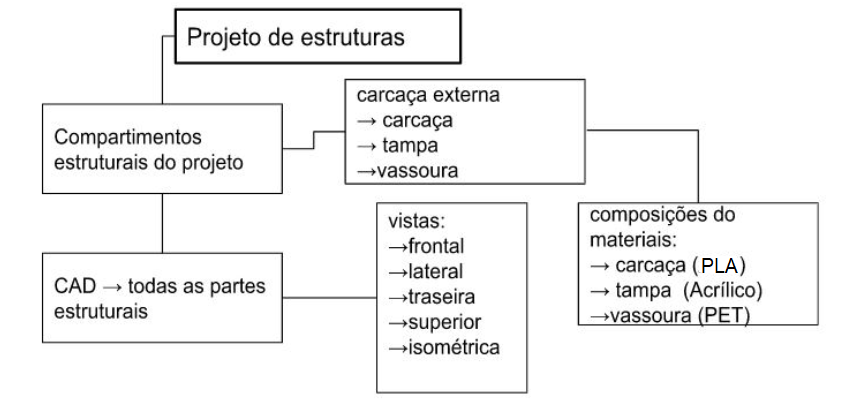
\includegraphics[scale=0.8]{figuras/estru.png}
\caption{Diagrama Estrutural\\ Fonte: Autoria própria, 2023}

\label{estru}
\end{figure}

Na tabela \ref{dim} tem-se as dimensões do Quirby, de forma que ela possa ser o mais compacto possível respeitando o espaço para a acomodação de todos os componentes, eletrônicos ou não, necessários para o funcionamento.

\begin{table}[h]
\centering
\caption{Dimensões do Robô\\Fonte: Autoria própria, 2023}
\label{dim}
\begin{tabular}{|
>{\columncolor[HTML]{FFFFFF}}l |
>{\columncolor[HTML]{FFFFFF}}r |lll}
\cline{1-2}
Dimensão Estrutural         & \textit{mm} \multicolumn{1}{l|} {\cellcolor[HTML]{FFFFFF}} &  &  &  \\ \cline{1-2}
Diâmetro                        & \textit{300}                                  &  &  &  \\ \cline{1-2}
Espessura da tampa e da carcaça & \textit{2,5}                                    &  &  &  \\ \cline{1-2}
Altura                          & \textit{86,6}                                   &  &  &  \\ \cline{1-2}
\end{tabular}
\end{table}

As vassouras do robô são feitas de PET (Polietileno tereftalato) de densidade baixa na qual é um termoplástico semi cristalino e amorfo, com propriedade de tração mecânica baixa.Na figura \ref{vass} pode-se ver o CAD da vassoura do "Quirby".

\begin{figure}[h!]
\includegraphics[height=3.8 cm, width=16 cm]{figuras/Vassoura1.jpg}
\caption{Vassoura \\ Fonte: Autoria própria, 2023}
\label{vass}
\end{figure}



\\
\\

Como visto na figura \ref{estru}, a carcaça do robô é feita de PLA (Ácido Polilático latico), que é um ácido orgânico de origens naturais como amido de milho ou cana-de-açúcar.
Na figura \ref{fig1} pode-se observar a imagem mais refinada de como o "Quirby" se apresentará ao fim do projeto.
\begin{figure}[h!]
\begin{center}
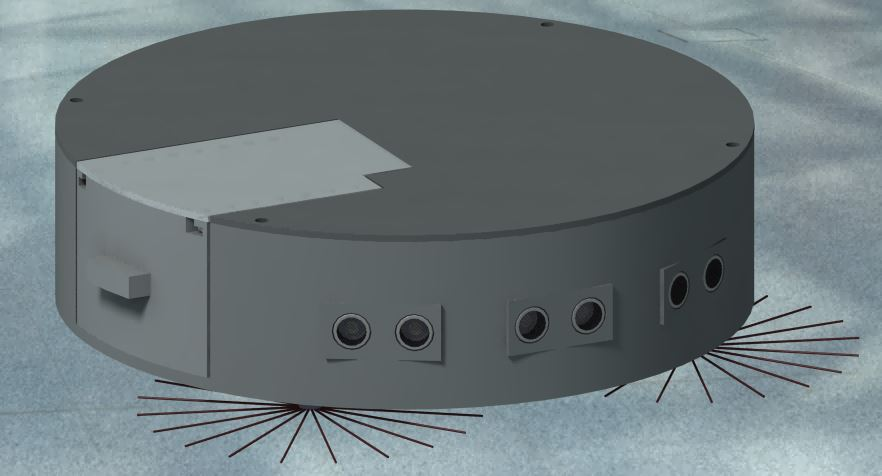
\includegraphics[width=0.5\textwidth]{figuras/isometrica.jpg}
\caption{Carcaça \\ Fonte: Autoria própria, 2023}
\label{fig1}
\end{center}
\end{figure}

A Tampa do Compartimento de pó é feita de acrílico, um termoplástico na qual apresenta um alto nível de transparência, atóxico e resistente a intempéries. Na figura \ref{tampa} tem-se uma representação da tampa de acrílico do reservatório de dejetos do "Quirby".

\begin{figure}[h]
\begin{center}
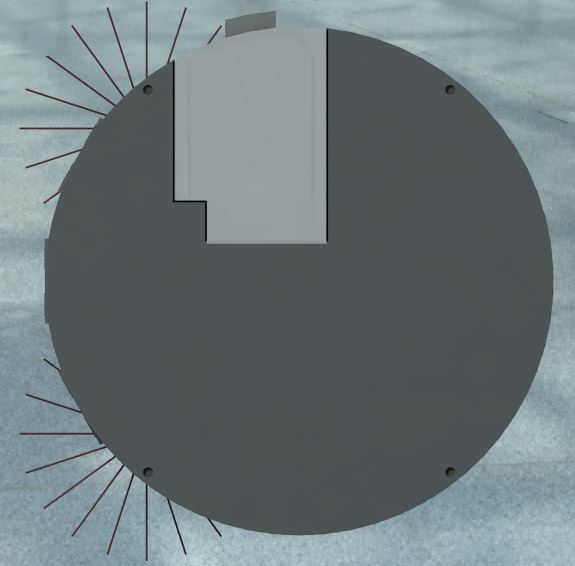
\includegraphics[width=0.3\textwidth]{figuras/superior.jpg}
\caption{Tampa do Compartimento\\Fonte: Autoria própria, 2023}
\label{tampa}
\end{center}
\end{figure}

\subsection{Matriz de decisões - descrição geral dos critérios de seleção do produto
}

Nas tabelas \ref{tabprop} e \ref{tabter} tem-se as propriedades mecânicas e térmicas dos materiais escolhidos para compor o "Quirby".
\\
\begin{table}[h]
\centering
\caption{Propriedas Mecânicas dos Materias\\Fonte: enge-materiais.bh, 2023}
\label{tabprop}
\begin{tabular}{|
>{\columncolor[HTML]{FFFFFF}}l |
>{\columncolor[HTML]{FFFFFF}}l |}
\hline
\textbf{Materiais} & \textbf{Propriedades Mecânicas}                                                      \\ \hline
\textbf{PLA}       & leve e fácil de moldar, resistência ao desgaste                        \\ \hline
\textbf{Acrílico}  & resistência ao desgaste, pouco flexível e transparente                                 \\ \hline
\textbf{PET}       & {\color[HTML]{202124} pouca resistência à tração, comportamento deslizante e dureza} \\ \hline
\end{tabular}
\end{table}
\\
\\
\begin{table}[h]
\centering
\caption{Propriedades Térmicas dos Materiais\\Fonte: enge-materiais.bh, 2023}
\label{tabter}
\begin{tabular}{|
>{\columncolor[HTML]{FFFFFF}}l |
>{\columncolor[HTML]{FFFFFF}}l |
>{\columncolor[HTML]{FFFFFF}}l |}
\hline
\textbf{Materiais} & \textbf{Composição} & \textbf{Propriedades Térmicas} \\ \hline
\textbf{PLA}       & Poliácido latico    & entre 55°C-65 °C                \\ \hline
\textbf{Acrílico}  & Termoplástico       & entre 60°C-93 °C                \\ \hline
\textbf{PET}       & Termoplástico       & até 70 °C             \\ \hline
\end{tabular}

\end{table}

\\
 O material escolhido foi o PLA, levando-se em consideração a limitação do orçamento, além do tipo de impressora 3D disponível para uso.
\\
 \begin{figure}[h]
\begin{center}
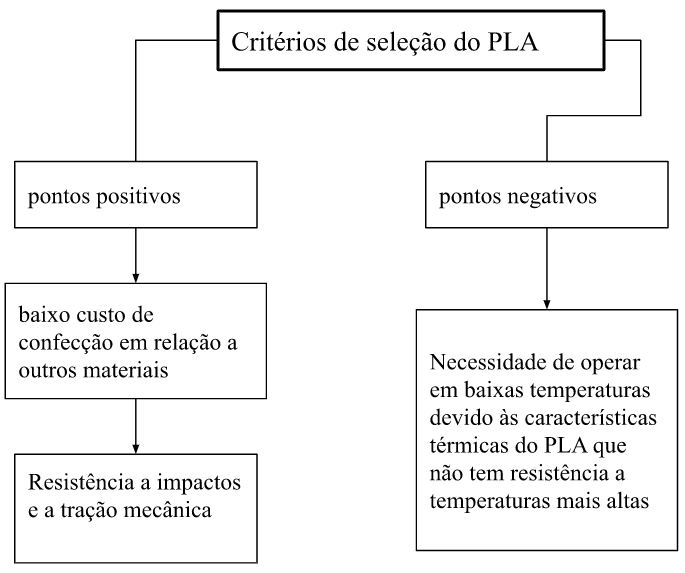
\includegraphics[width=0.65\textwidth]{figuras/pla_crite.jpg}
\caption{PLA - critérios de seleção\\Fonte: Autoria própria, 2023}
\label{tampa}
\end{center}
\end{figure}

A escolha do acrílico para a tampa foi com base na sua resistência a intempéries e a sua facilidade de modulação, a sua resistência ao intemperismo serve de proteção contra degastes e sua modulação ajuda na ajuste entre as partes das peças.
 \begin{figure}[h]
\begin{center}
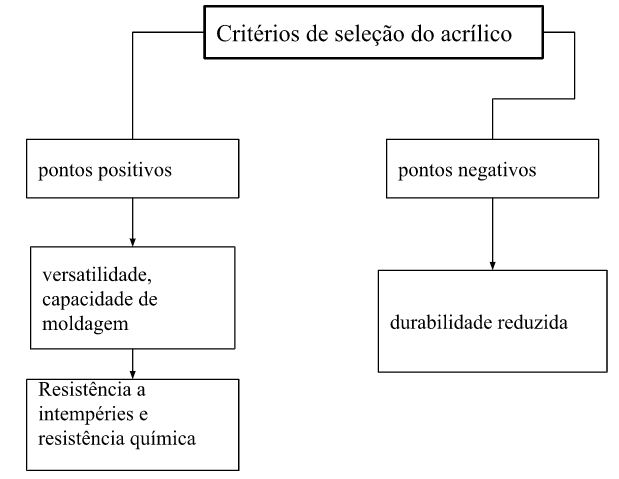
\includegraphics[width=0.65\textwidth]{figuras/acri_crite.jpg}
\caption{Acrílico - critérios de seleção\\Fonte: Autoria própria, 2023}
\label{tampa}
\end{center}
\end{figure}
\newpage
\pagebreak
A escolha do material PET na vassoura do robô foi com base seu baixo desgaste, a sua baixa absorção de umidade e o seu comportamento deslizante
\\
 \begin{figure}[h]
\begin{center}
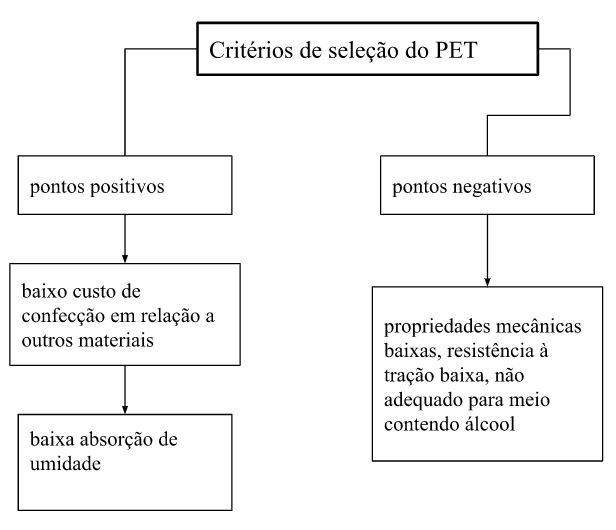
\includegraphics[width=0.5\textwidth]{figuras/pet_diagrama.jpg}
\caption{PET - critérios de seleção\\Fonte: Autoria própria, 2023}
\label{tampa}
\end{center}
\end{figure}

A integração da escolha desses materiais; PET, acrílico, PLA tem como objetivo o baixo custo em ambos os 3 materiais, suas propriedades mecânicas foram pensadas na melhor compatibilidade em prol da integração.

 \begin{figure}[h]
\begin{center}
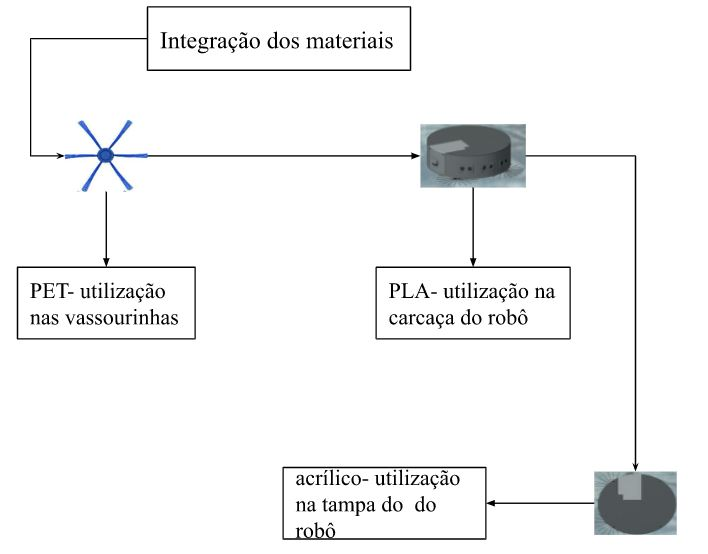
\includegraphics[height=6 cm, width=14 cm]{figuras/intemat.jpg}
\caption{Integração dos materiais\\Fonte: Autoria própria, 2023}
\label{tampa}
\end{center}
\end{figure}
A escolha dos materiais é pautada no custo econômico de fabricação, consequentemente alterando o valor do produto.
\newpage
\pagebreak
 
\subsection{CAD Estrutural}
O CAD(\textit{Computer-Aided Design}) estrutural do Quirby é composto por suas vistas, nas quais são separadas em vistas: isométrica, lateral, traseira, superior, superior com componentes e isométrica com componentes, como pode-se observar nas figuras \ref{vistaFrontal} a \ref{fig:subfig}:
\\

\begin{figure}[h!]
\centering
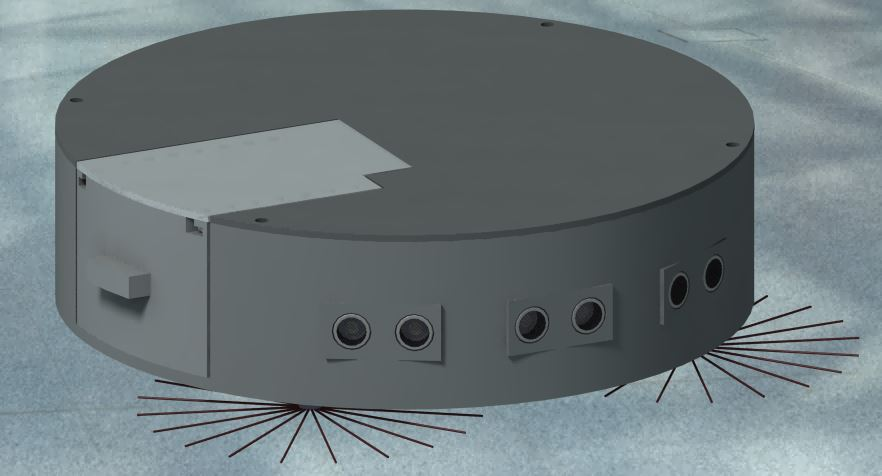
\includegraphics[width=0.5\textwidth]{figuras/frontal.jpg}
\caption{Vista isométrica\\Fonte: Autoria própria, 2023}
\label{vistaFrontal}
\end{figure}
 A vista isométrica mostra a parte superior frontal e lateral do robô, sendo possível observar os materiais de utilizados no projeto.
\\
\\
\begin{figure}[h!]
\centering
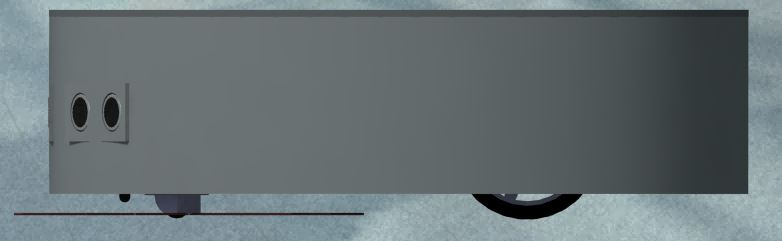
\includegraphics[width=0.5\textwidth]{figuras/direita.jpg}
\caption{Vista lateral direita\\Fonte: Autoria própria, 2023}
\label{vistaLateral}
\end{figure}


A vista lateral direita do robô permite a visualização dos demais componentes presentes no robô, tais como as vassouras, rodas e sensor LED, etc.
\\
\newpage
\pagebreak
\begin{figure}[h!]
\centering
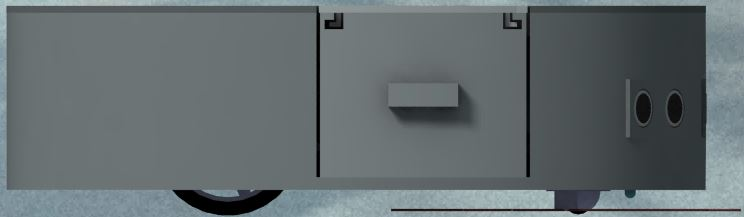
\includegraphics[width=0.5\textwidth]{figuras/esquerda.jpg}
\caption{Vista lateral esquerda\\Fonte: Autoria própria, 2023}
\label{vistaLateral}
\end{figure}

A vista lateral esquerda do robô facilita a observação do compartimento do pó, bem como outras partes do projeto.
\\
\begin{figure}[h!]
\centering
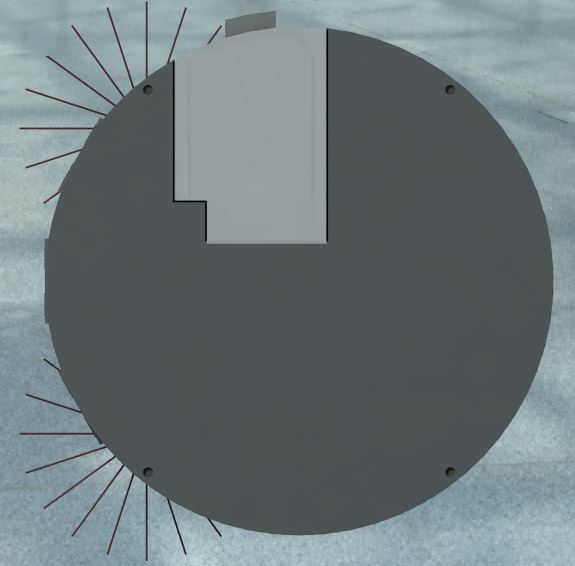
\includegraphics[width=8cm,height=4cm]{figuras/superior.jpg}
\caption{Vista superior\\Fonte: Autoria própria, 2023}
\label{vistaLateral}
\end{figure}


 A vista superior do robô mostra a tampa do compartimento e a tampa da carcaça. 
 \\
 \\
\begin{figure}[h!]
\centering
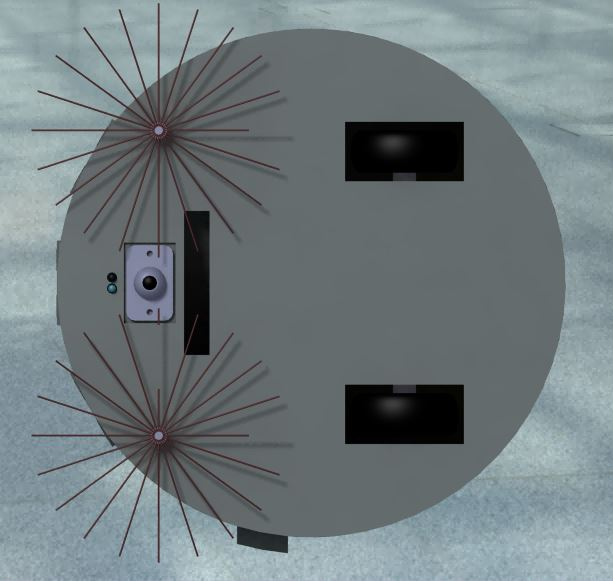
\includegraphics[width=8cm,height=6cm]{figuras/inferior.jpg}
\caption{Vista inferior\\Fonte: Autoria própria, 2023}
\label{vistaLateral}
\end{figure}


Na visão da parte inferior do robô têm-se as rodas, tanto motoras quanto a roda boba, há também as vassouras e a abertura de aspiração.

\newpage
\pagebreak
Na figura \ref{fig:subfig} é possível observar a acomodação dos componentes eletrônicos na estrutura interna do robô, seguida da tabela de legenda.
\\
\begin{figure}[h!]
\centering
\subfloat{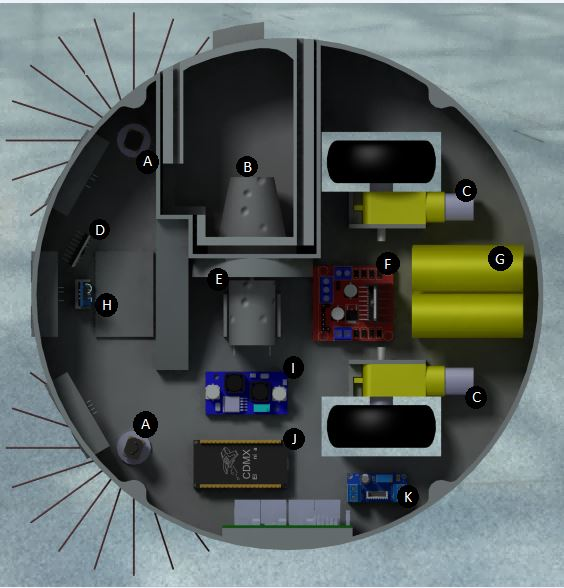
\includegraphics[width=7cm,height=8cm]{figuras/superiorcomp.jpg}
}
\hfill
\subfloat{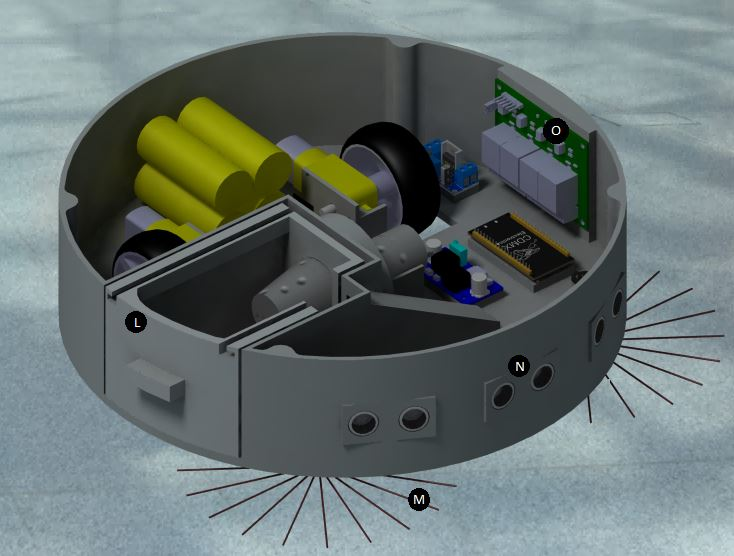
\includegraphics[width=7cm,height=8cm]{figuras/isometrica_comp.jpg}}
\caption{Vistas superior e isométrica com componentes:\\Fonte: Autoria própria, 2023}
\label{fig:subfig}
\end{figure}

\begin{table}[h]
    \centering
    \caption{Lista de componentes\\Fonte: Autoria própria, 2023}
    \label{tab:my_label}
    \begin{tabular}{|c|c|}
    \hline
    & Componentes\\ \hline
    A & Mini Motor DC N20 com Caixa de Redução 6V 100 RPM \\ \hline
    B & Filtro HEPA \\ \hline
    C & Motor DC 6V com caixa de redução e Roda \\ \hline
    D & MPU 6050 \\ \hline
    E & Motor DC 12V Aspirador \\ \hline
    F & Driver Motor Ponte H L298N \\ \hline
    G & Baterias 26650 3.7V 5000mAh \\ \hline
    H & Módulo Sensor de Reflexão IR c/ Fotodiodo \\ \hline
    I & Conversor DC-DC Step UP XL6009 \\ \hline
    J & Esp32 Wifi Wroom-32 \\ \hline
    K & Conversor DC-DC Step Down Lm317 \\ \hline
    L & Recipiente de armazenamento de Pó \\ \hline
    M & Vassouras \\ \hline
    N & Sensor Ultrassônico HC-SR04 \\ \hline
    O & Módulo Relê 5V 10A \\ \hline
    \end{tabular}
\end{table}

\newpage
\pagebreak
\subsection{Desenhos Técnicos}
As imagens a seguir (Figuras \ref{CapaInferior1_4} a \ref{Tampa_Compartimento}) referem-se aos desenhos técnicos do Quirby, sendo válida a seguinte observação: dado tamanho da carcaça externa e seu elevado número de subestruturas, teve-se que dividir a carcaça em quatro partes, das quais estão representadas nas imagens abaixo. Sendo assim, as medidas de cada subestrutura consta em uma das 4 partes, não havendo necessidade de repetir cotas para uma mesma subestrutura.


Para que haja melhor resolução e possibilite a identificação das cotas do projeto, inseriu-se uma imagem por página.

\newpage
\pagebreak
\begin{figure}[h!]
\centering
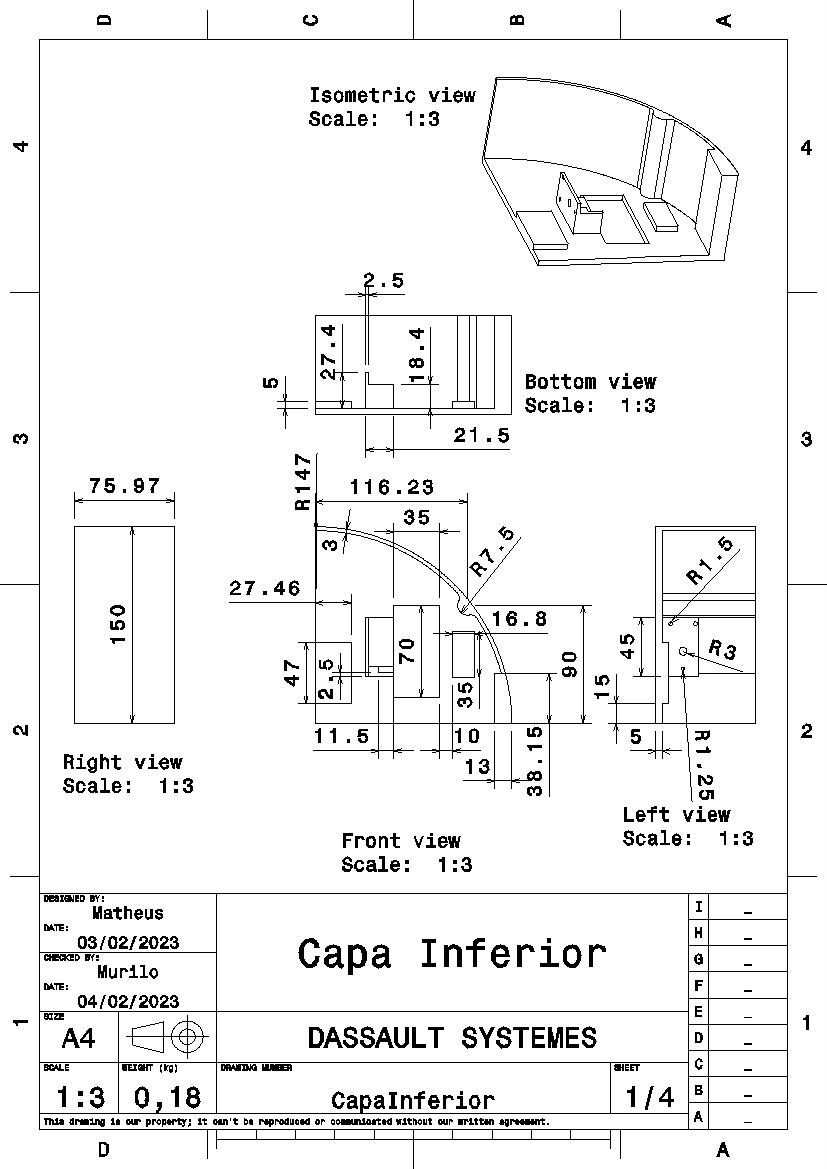
\includegraphics[width=16cm,height=22cm]{figuras/CapaInferior1_4.jpg}
\caption{Capa inferior 1/4\\Fonte: Autoria própria, 2023}
\label{CapaInferior1_4}
\end{figure}

\newpage
\pagebreak
\begin{figure}[h!]
\centering
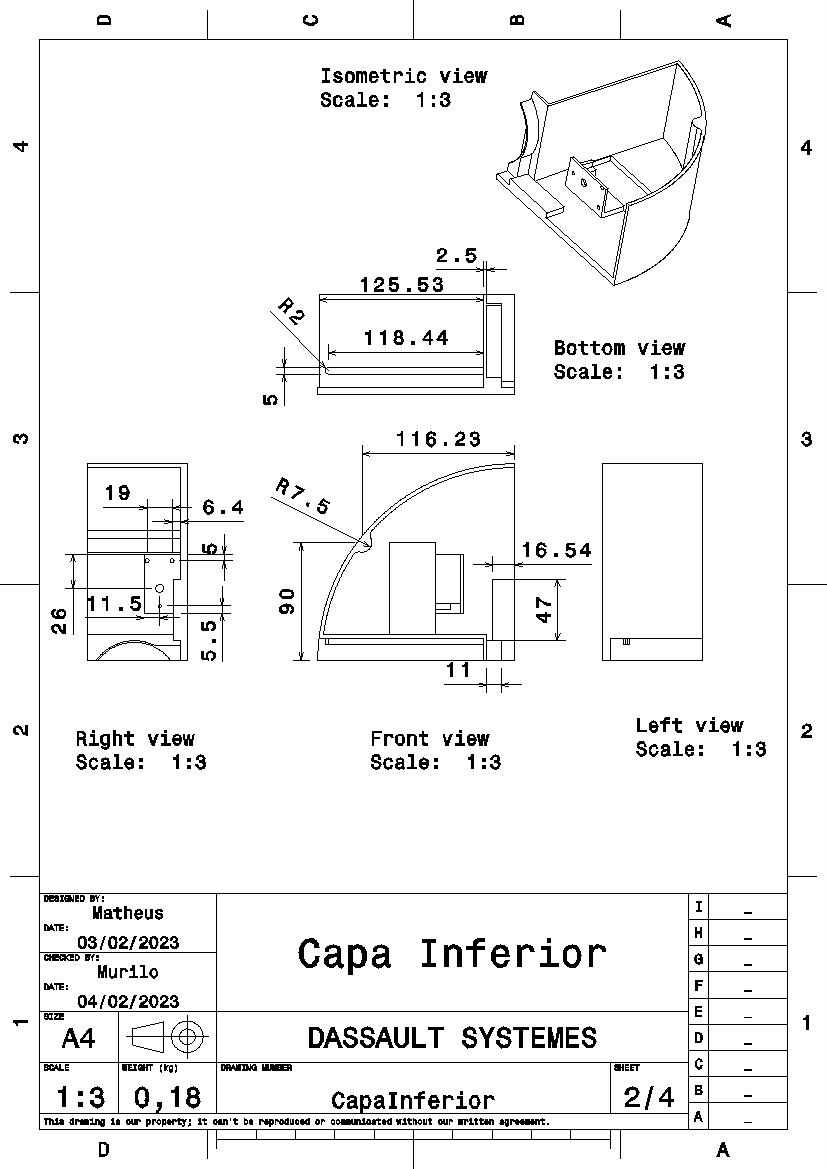
\includegraphics[width=16cm,height=22cm]{figuras/CapaInferior2_4.jpg}
\caption{Capa inferior 2/4\\Fonte: Autoria própria, 2023}
\label{CapaInferior2_4}
\end{figure}

\newpage
\pagebreak
\begin{figure}[h!]
\centering
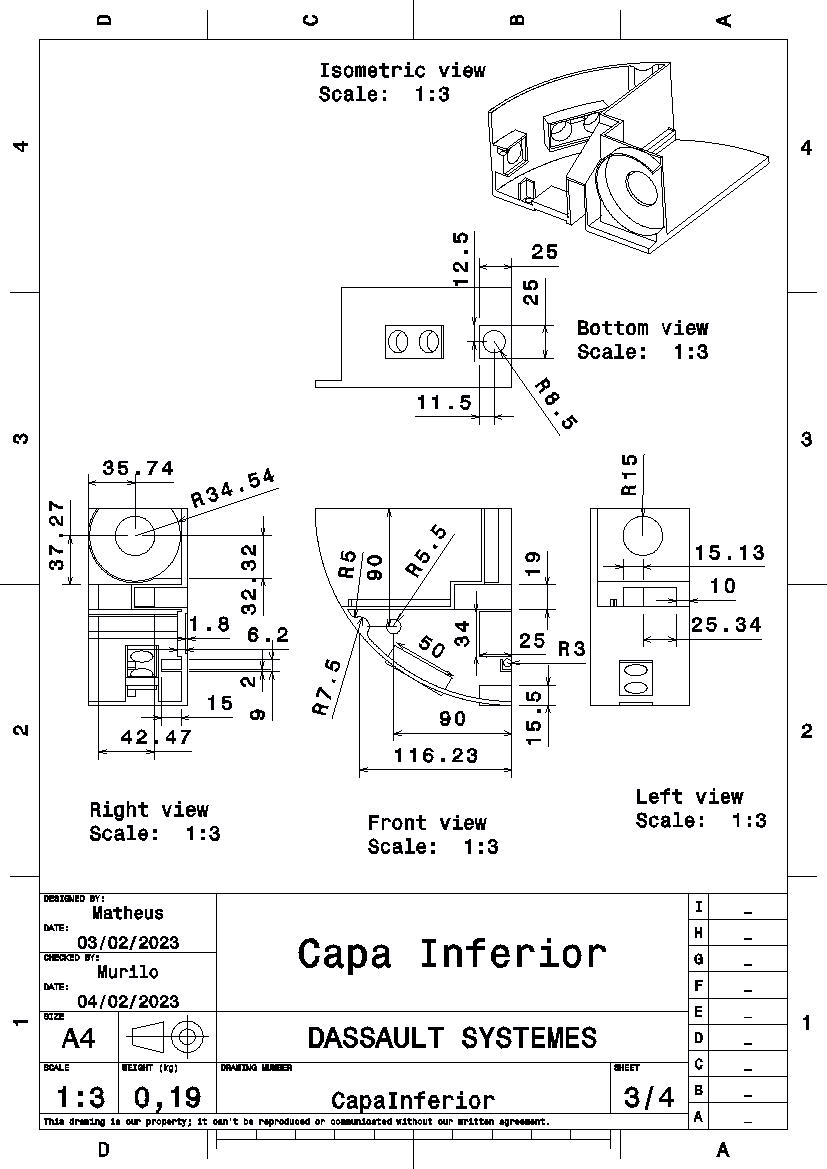
\includegraphics[width=16cm,height=22cm]{figuras/CapaInferior3_4.jpg}
\caption{Capa inferior 3/4\\Fonte: Autoria própria, 2023}
\label{CapaInferior3_4}
\end{figure}

\newpage
\pagebreak
\begin{figure}[h!]
\centering
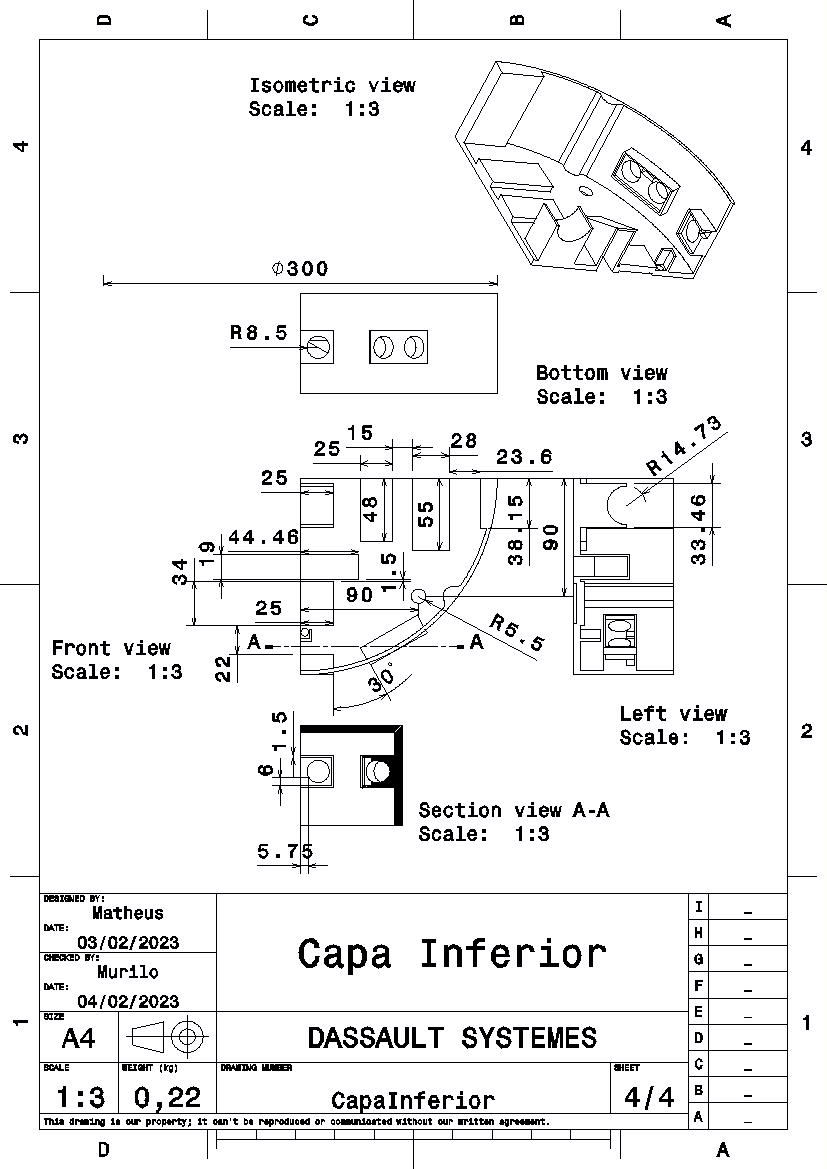
\includegraphics[width=16cm,height=22cm]{figuras/CapaInferior4_4.jpg}
\caption{Capa inferior 4/4\\Fonte: Autoria própria, 2023}
\label{CapaInferior4_4}
\end{figure}

\newpage
\pagebreak
\begin{figure}[h!]
\centering
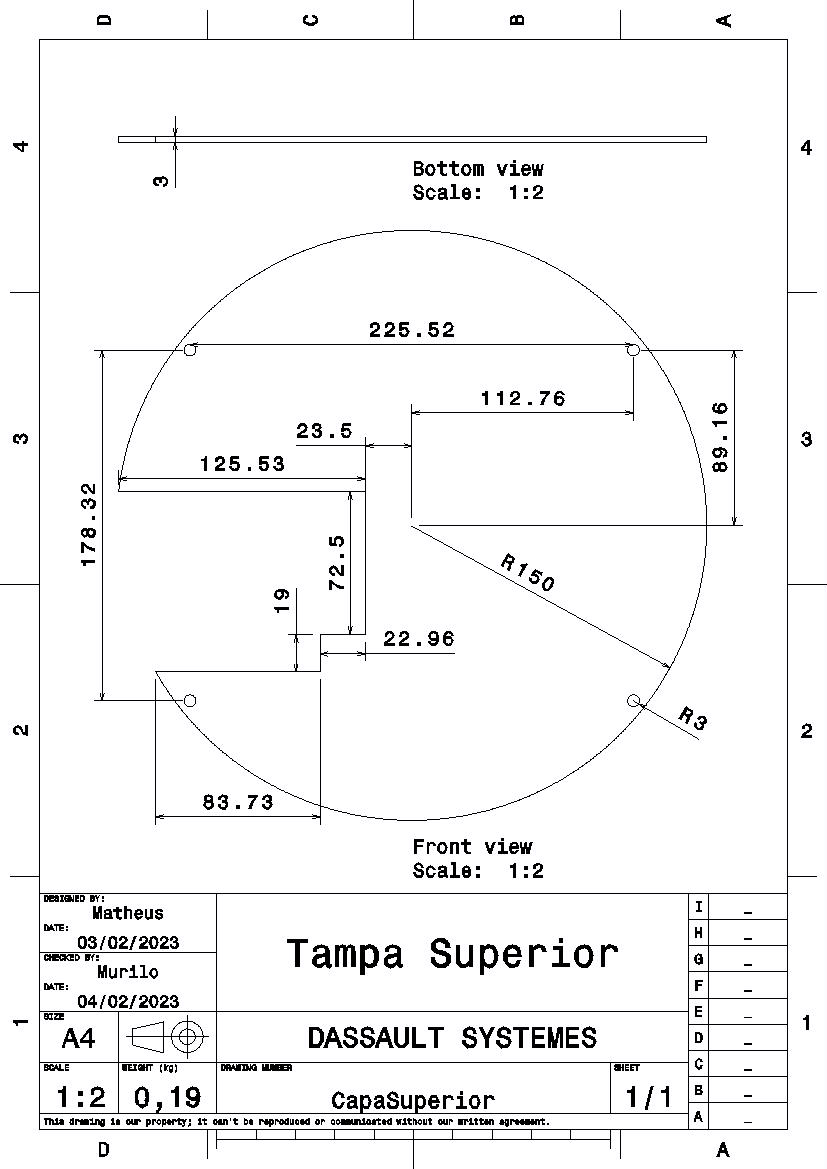
\includegraphics[width=16cm,height=22cm]{figuras/Tampa_Superior.jpg}
\caption{Tampa superior\\Fonte: Autoria própria, 2023}
\label{Tampa_Superior}
\end{figure}

\newpage
\pagebreak
\begin{figure}[h!]
\centering
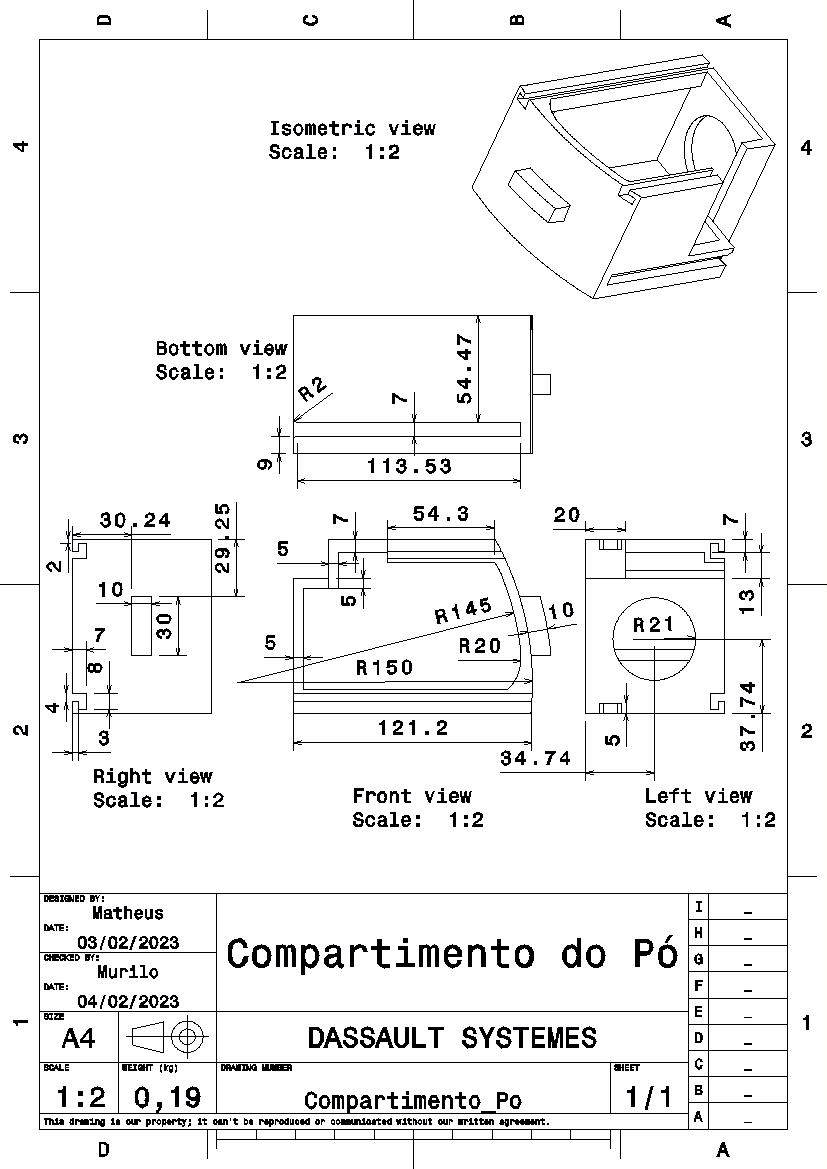
\includegraphics[width=16cm,height=22cm]{figuras/Compartimento_Po.jpg}
\caption{Compartimento de pó\\Fonte: Autoria própria, 2023}
\label{Compartimento_Po}
\end{figure}

\newpage
\pagebreak
\begin{figure}[h!]
\centering
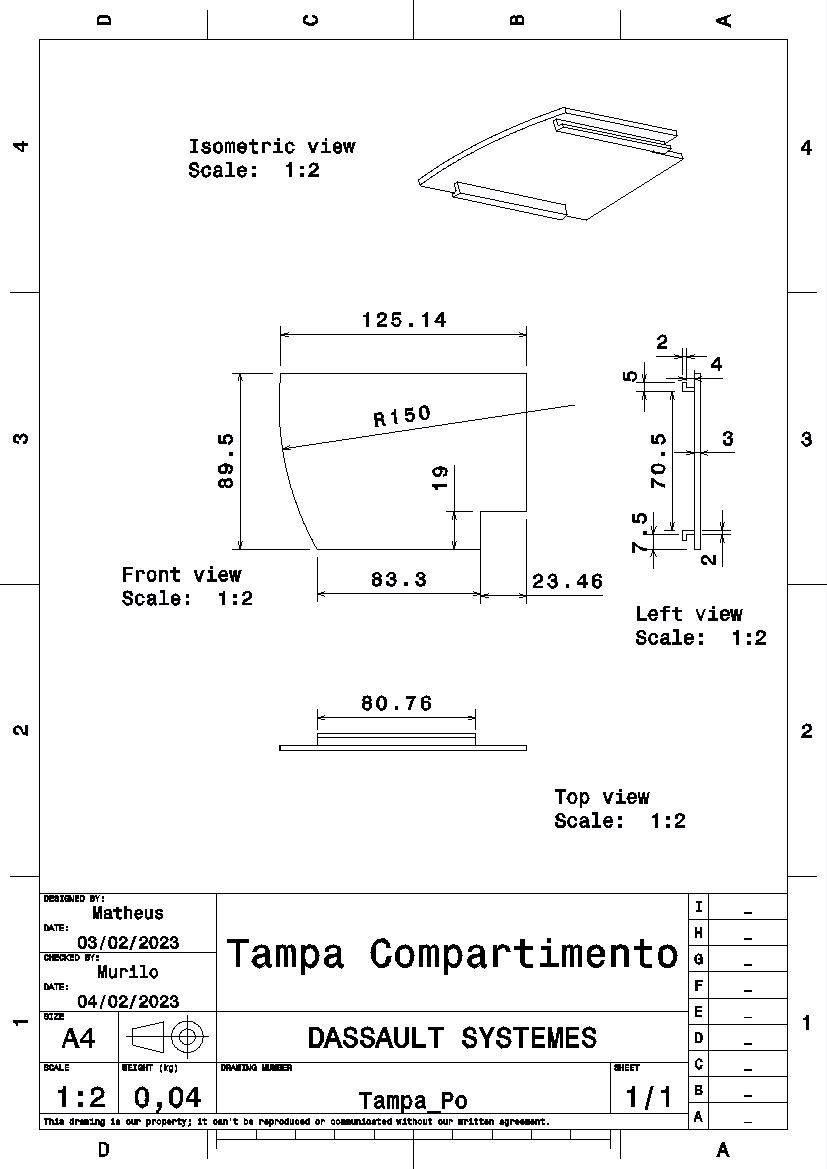
\includegraphics[width=16cm,height=22cm]{figuras/Tampa_Compartimento.jpg}
\caption{Tampa do compartimento\\Fonte: Autoria própria, 2023}
\label{Tampa_Compartimento}
\end{figure}

%\subsection{Elemento 1}

 

%\subsection{Elemento 2}
% Detalhar o projeto do elemento 02 do subsistema.
% Criar mais se necessário
\newpage
\pagebreak
\clearpage
\section{Projeto de Eletrônica}

A solução eletrônica do projeto consiste em desenvolver sistemas para a movimentação, sensoriamento, alimentação do sistema e regulação de tensão para se adequar à cada componente, e será detalhada adiante.
\subsection{Representação esquemática das ligações dos componentes} 
% Detalhar o projeto do elemento 01 do subsistema. 
Com a definição dos componentes para a aplicação do projeto, foi desenvolvido o esquema de ligação dos componentes com o microcontrolador ESP-32\cite{ESPRESSIFMANUAL}, para recebimento dos sinais dos sensores e acionamento dos atuadores e todo o sistema de alimentação dos componentes, onde para sua maioria é necessária uma tensão de 5V.

\begin{figure}[H]
\centering
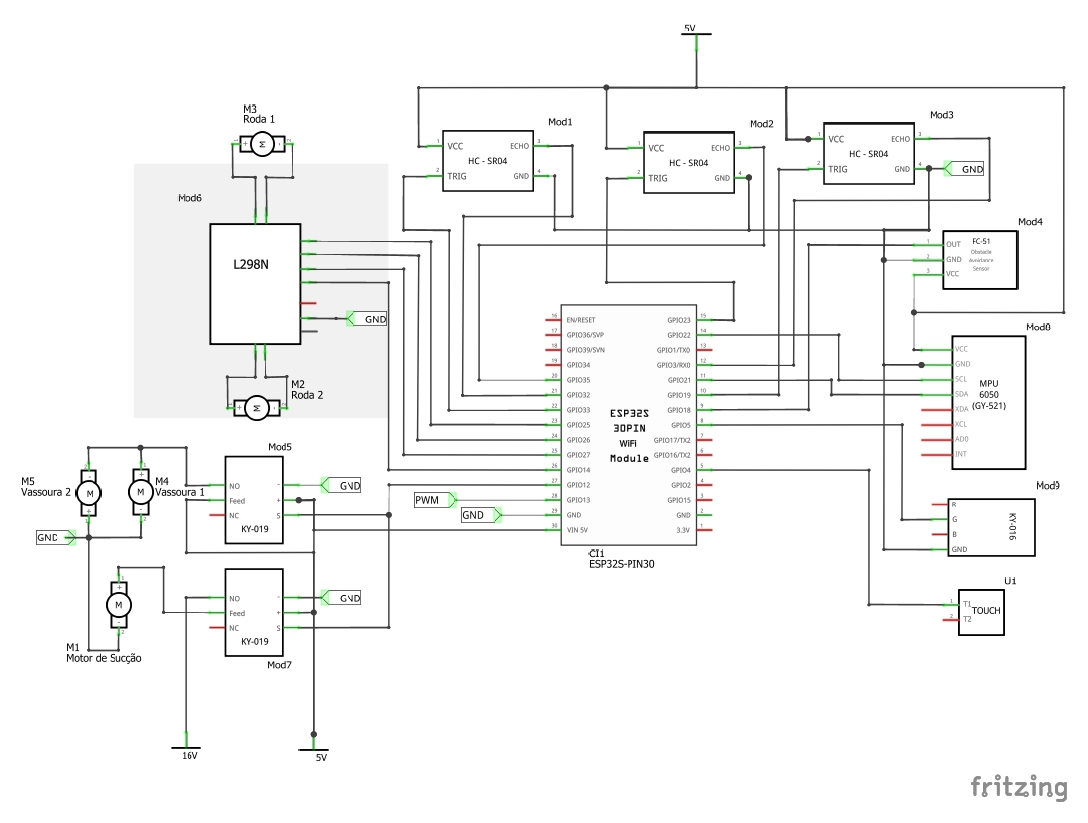
\includegraphics[width=1.0\textwidth]{editaveis/aa.jpg}
\caption{Representação esquemática dos componentes eletrônicos e suas conexões \\ Fonte: Autoria própria, 2023}

\label{eletroesq}
\end{figure}

O diagrama expresso na figura \ref{eletroesq} representa as conectividades entre os componentes eletrônicos empregados no projeto. Os componentes envolvem sensores, motores e módulos de controle de carga indutiva. Os componentes expressos na figura \ref{eletroesq} são:
\begin{itemize}
    \item \textbf{Motores}
    \begin{itemize}
    \item 1 Motor DC 16 volts (usado para sucção de partículas)
    \item 2 Motores DC 5 volts (usados para as vassouras)
    \item 2 Motores DC 5 volts (usados para tracionar as rodas do robô)
    \end{itemize}
    
    \item \textbf{Sensores}
\begin{itemize}
    \item 1 Sensor Infravermelho (FC-51) (usado para evitar quedas do dispositivo)
    \item 3 Sensores ultrassônicos (HC-SR04) (usados para detecção de obstáculos)
    \item 1 Giroscópio (MPU-6050) (usado para detectar velocidade angular nos 3 eixos)
\end{itemize}
    \item \textbf{Alimentação}
\begin{itemize}
    \item 1 Pack de Baterias 4S (16,8 Volts e 5000mAh)
    \item 1 Regulador de tensão (16.8V para 5V) (para alimentação de todos os componentes exceto motor de sucção)
\end{itemize}
    \item \textbf{Componentes de Comando/Controle}
\begin{itemize}
    \item ESP32S 30PIN WIFI MODULE (Central de processamento)
    \item Ponte H (L298N) (usada para controle das rodas de tração)
\end{itemize}    
\end{itemize}


\subsection{Montagens iniciais}

A equipe realizou testes iniciais sobre o funcionamento dos componentes, o que demonstrou um resultado satisfatório para o estágio em que se encontra o projeto. Considerando que, apesar de o teste ter sido realizado sem a estrutura do robô, foi demonstrado o correto funcionamento dos componentes eletrônicos, tendo em vista que não houveram choques mecânicos e quedas em degraus. A montagem provisória realizada para teste inicial dos componentes eletrônicos está expressa na figura \ref{bocao}.
\begin{figure}[H]
\centering
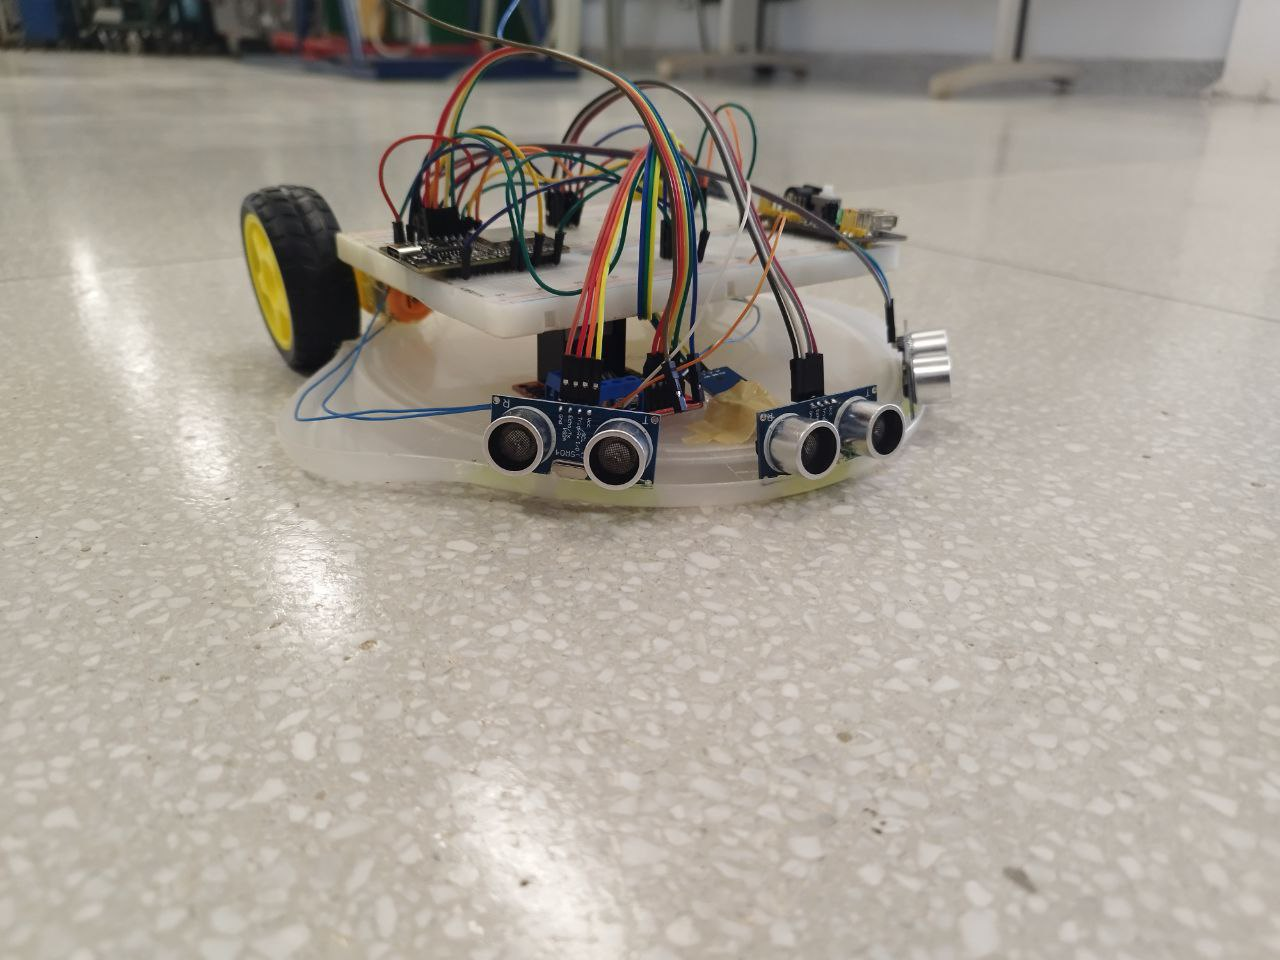
\includegraphics[width=0.7\textwidth]{editaveis/prot-inic.jpg}
\caption{Montagem provisória para teste de componentes eletrônicos}
\label{bocao}
\end{figure}

É possível observar a montagem preliminar para testes de movimentação e sensoriamento do ambiente do robô aspirador, onde foi possível fazer testes e calibragem de sensores e atuadores.

Posteriormente, com os componentes testados e calibrados, foi realizada a montagem dos componentes eletrônicos na estrutura definitiva do projeto, e é possível visualizar o resultado por meio da figura \ref{fig:bocao-montado}

\begin{figure}[!htb]
\centering
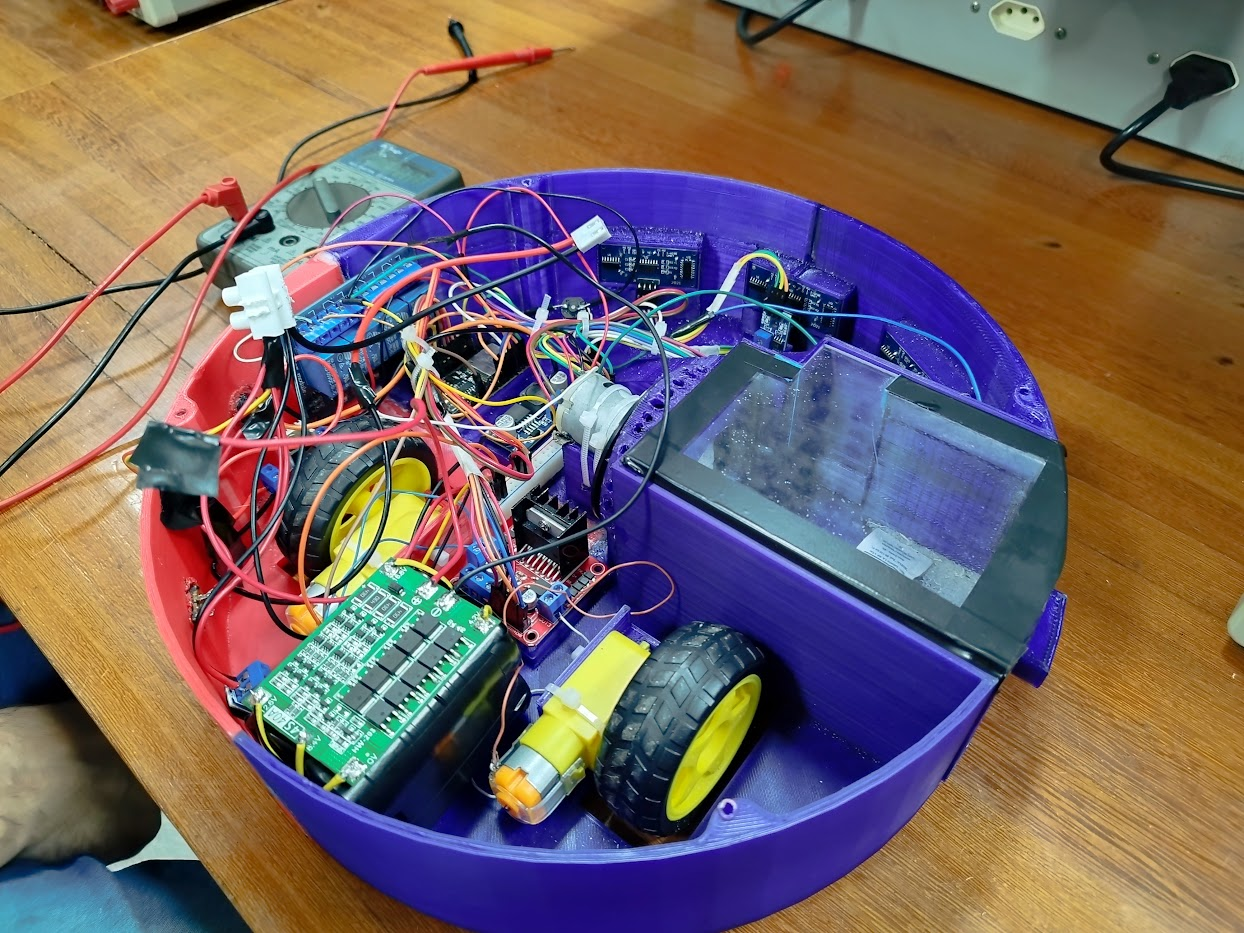
\includegraphics[width=0.7\textwidth]{editaveis/bocao-montado.jpg}
\caption{Montagem dos componentes na estrutura definitiva do projeto}
\label{fig:bocao-montado}
\end{figure}

\subsection{Alimentação do Sistema Eletrônico}

O sistema eletrônico possui uma alimentação de 16 e 5 V, onde os 16 volts são para alimentar o motor de sucção de pó e os 5 volts para alimentar o microcontrolador, os sensores e atuadores. A alimentação do robô é dada por baterias montando um  PACK com um Módulo Controlador BMS, que é um dispositivo eletrônico de segurança altamente recomendável para projetos que envolvam baterias de lítio, permitindo que a operação de carga e descarga seja devidamente monitorada e corrigida diante de algum problema. A montagem do PACK se deu pela configuração mostrada na figura \ref{bms}, onde se resulta em uma tensão de aproximadamente 16 volts.

\begin{figure}[H]
\centering
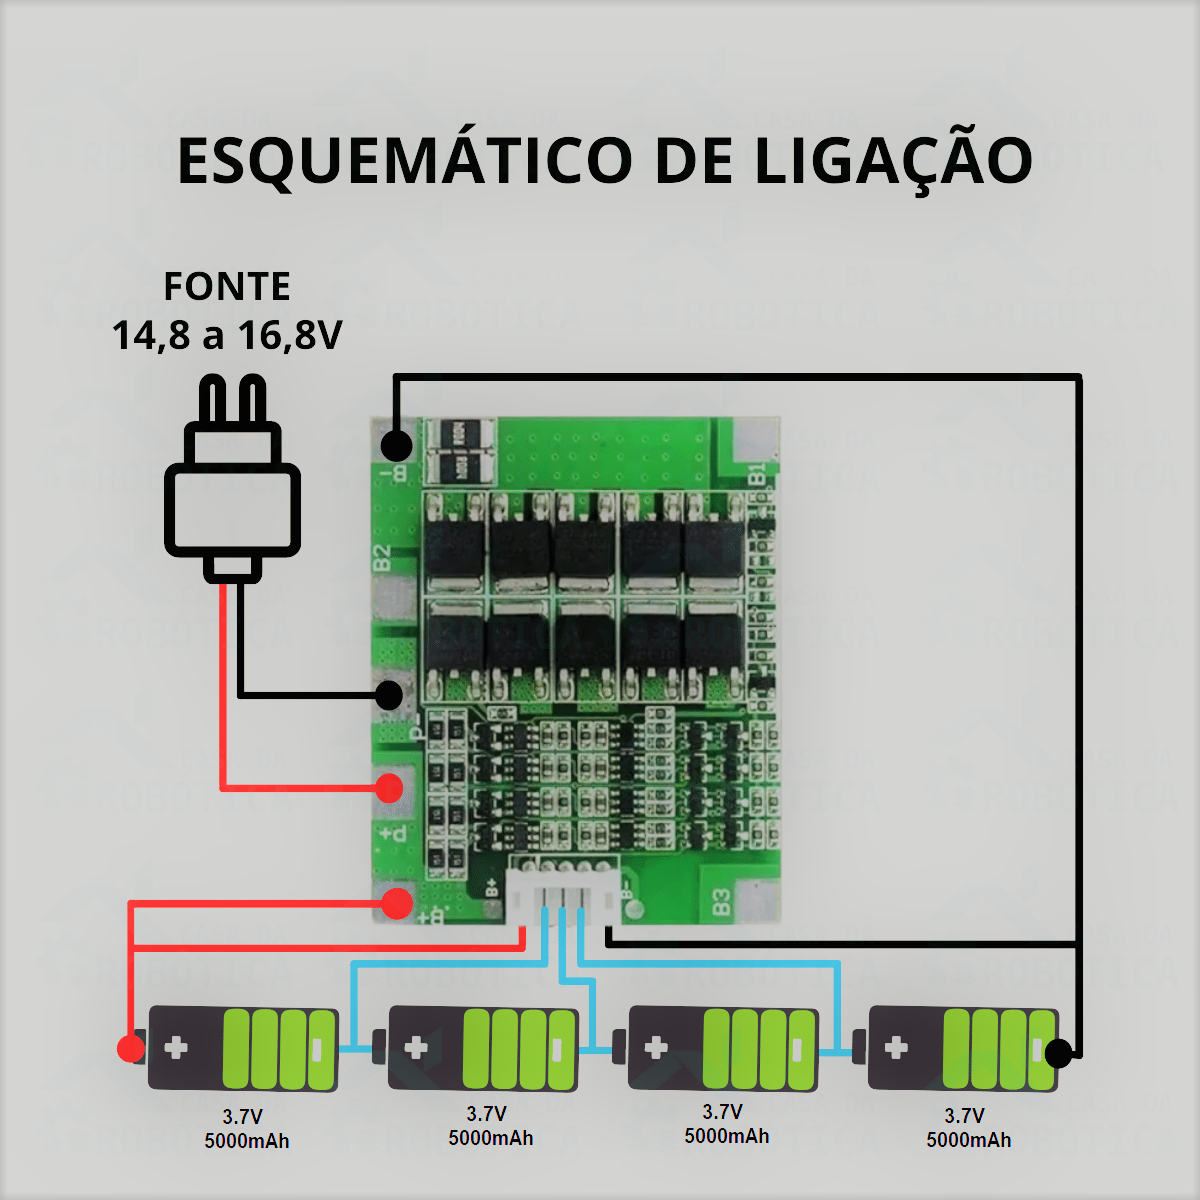
\includegraphics[width=0.5\textwidth]{editaveis/BMS.png}
\caption{Montagem elétrica do PACK de baterias}

\label{bms}
\end{figure}

É observado  na figura \ref{bms} que, para efetuar a recarga das baterias, é necessário aplicar uma diferença de potencial entre 14,8V e 16,8V na entrada. Para fazer a regulagem de tensão para obter os 5V desejado para alimentar todo o sistema é usado o modulo regulador de tensão Step-Down - Lm2596, onde é conectado na sua entrada a saída da bateria e, assim, regulando a tensão de saída de 16V para 5V.

\section{Projeto de Software}

A Solução de Software corresponde a um aplicativo \textit{mobile}, para Android 10 ou superior, que se comunica com o robô aspirador. A solução será detalhada a seguir.

\subsection{Backend} 

O Backend se refere à camada de Software não visível ao usuário, mas que apoia a camada visual \cite{ewally_2021}. O Backend do Quirby diz respeito ao servidor na nuvem que intermedeia a conexão entre o aplicativo Mobile e o robô. 

As tecnologias utilizadas são o Node.js que é um motor JavaScript orientado a eventos e assíncrono, o PostgreSQL que é um SGBD, o Docker que faz a containerização e, por fim, o Heroku, o serviço de hospedagem utilizado para a disponibilização do servidor.

São utilizados 2 contâiners Docker no servidor: um para a base de dados no PostgreSQL e outro para aplicação Node.

A base de dados no PostgreSQL possui duas entidades: Robô e Pessoa, ilustradas na Figura \ref{diagramaConceitual}, sendo as duas responsáveis por armazenar os dados e status de robôs (caso houvesse mais que um) e as informações de usuários respectivamente. O esquema de organização destas entidades em tabelas no Banco de Dados está disposto na Figura \ref{diagramaLogico}.  

\begin{figure}[h!]
\centering
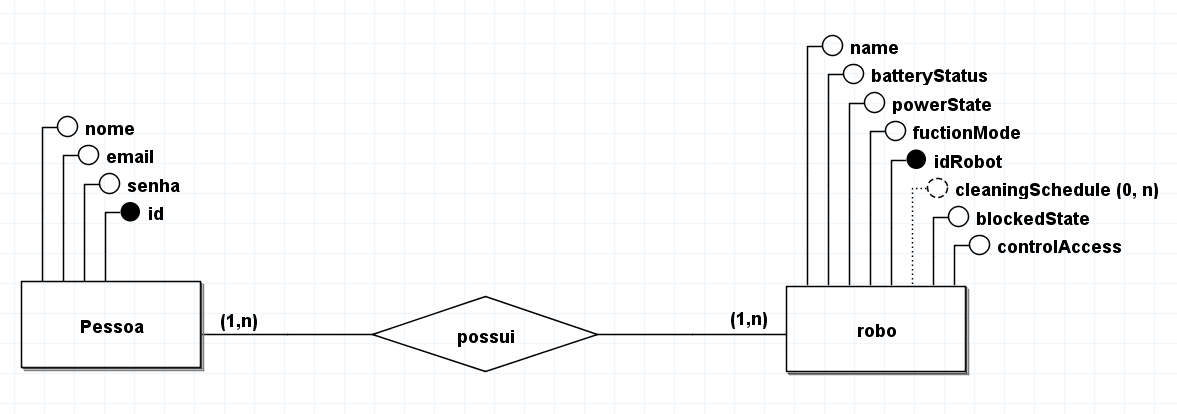
\includegraphics[scale=0.5]{figuras/software/Quiby_Diagrama_Conceitual.png}
\caption{Diagrama Conceitual de Banco de Dados \\ Fonte: Autoria própria, 2023}
\label{diagramaConceitual}
\end{figure}

\begin{figure}[h!]
\centering
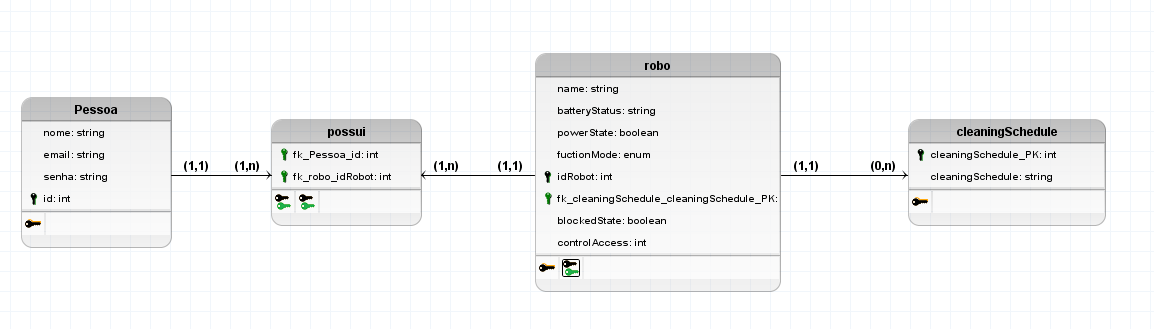
\includegraphics[scale=0.5]{figuras/software/Quirby_Diagrama_Logico.png}
\caption{Diagrama Lógico de Dados \\ Fonte: Autoria própria, 2023}
\label{diagramaLogico}
\end{figure}


Já a aplicação Node serve como a central e recebe as requisições, fazendo a comunicação com o aplicativo Mobile e com o robô, e interage com a base de dados utilizando como ORM o Sequelize.

% (Falar das rotas?)

Para a criação e autenticação das contas de usuário é utilizada a API do Google com o protocolo  OAuth 2.0. Desta forma o usuário deve fazer login com sua conta Google e o servidor fica responsável apenas por verificar se o usuário já está presente na base, e cadastrá-lo, caso contrário.


\subsection{Frontend}

O Frontend refere-se a interface da solução com a qual usuário irá interagir diretamente para possibilitar a execução dos comandos desejados no aplicativo mobile. 

A interface gráfica da solução é construída utilizando a linguagem de programação Dart, a partir da utilização do framework Flutter. Optou-se pela utilização do Flutter, por ser um framework gratuito de código aberto e que permite desenvolvimento móvel multiplataforma \cite{alberto_2022}. 
    
O Apêndice \ref{prototipo} apresenta as telas do protótipo de Baixa-Média fidelidade associadas ao design visual da solução, elaboradas com auxílio da ferramenta Figma.


\subsection{Firmware}

Para o Firmware, será utilizado o framework da própria empresa da Espressif Systems, a Espressif IoT Development Framework (ESP-IDF) \cite{ESPRESSIFMANUAL}, sendo que seu uso consegue explorar na totalidade os recursos vindo do microprocessador ESP32. Dando ênfase a arquitetura do software, visamos a apresentação do diagrama de classes, referenciando o nível mais baixo de comunicação entre os dispositivos em cada IO do MCU, controle das operações, e protocolos de comunicação entre o servidor e o aplicativo. 

Conforme a Figura \ref{diagramaClasseFirm}, as entradas e saídas dos dispositivos usados serão os primeiros a serem inicializados no software com os pinos definidos em cada classe de enumeração. Em seguida são instanciados os protocolos de comunicação, que irão manter a conexão via rede local por Wi-Fi e também pelo dispositivo pareado via Bluetooth. Posteriormente às dependências instanciadas, serão criadas tarefas divididas em cada subsistema, que envolve a operação dos movimentos do robô, sensores que evitam colisões e quedas e a comunicação externa.

Por fim, a classe Control faz toda a inclusão e gerenciamento desses subsistemas, sendo a primeira tarefa a ser instanciada no sistema. Com isso, temos o funcionamento de todo o sistema que envolve controle e comunicação.

\begin{figure}[h!]
\centering
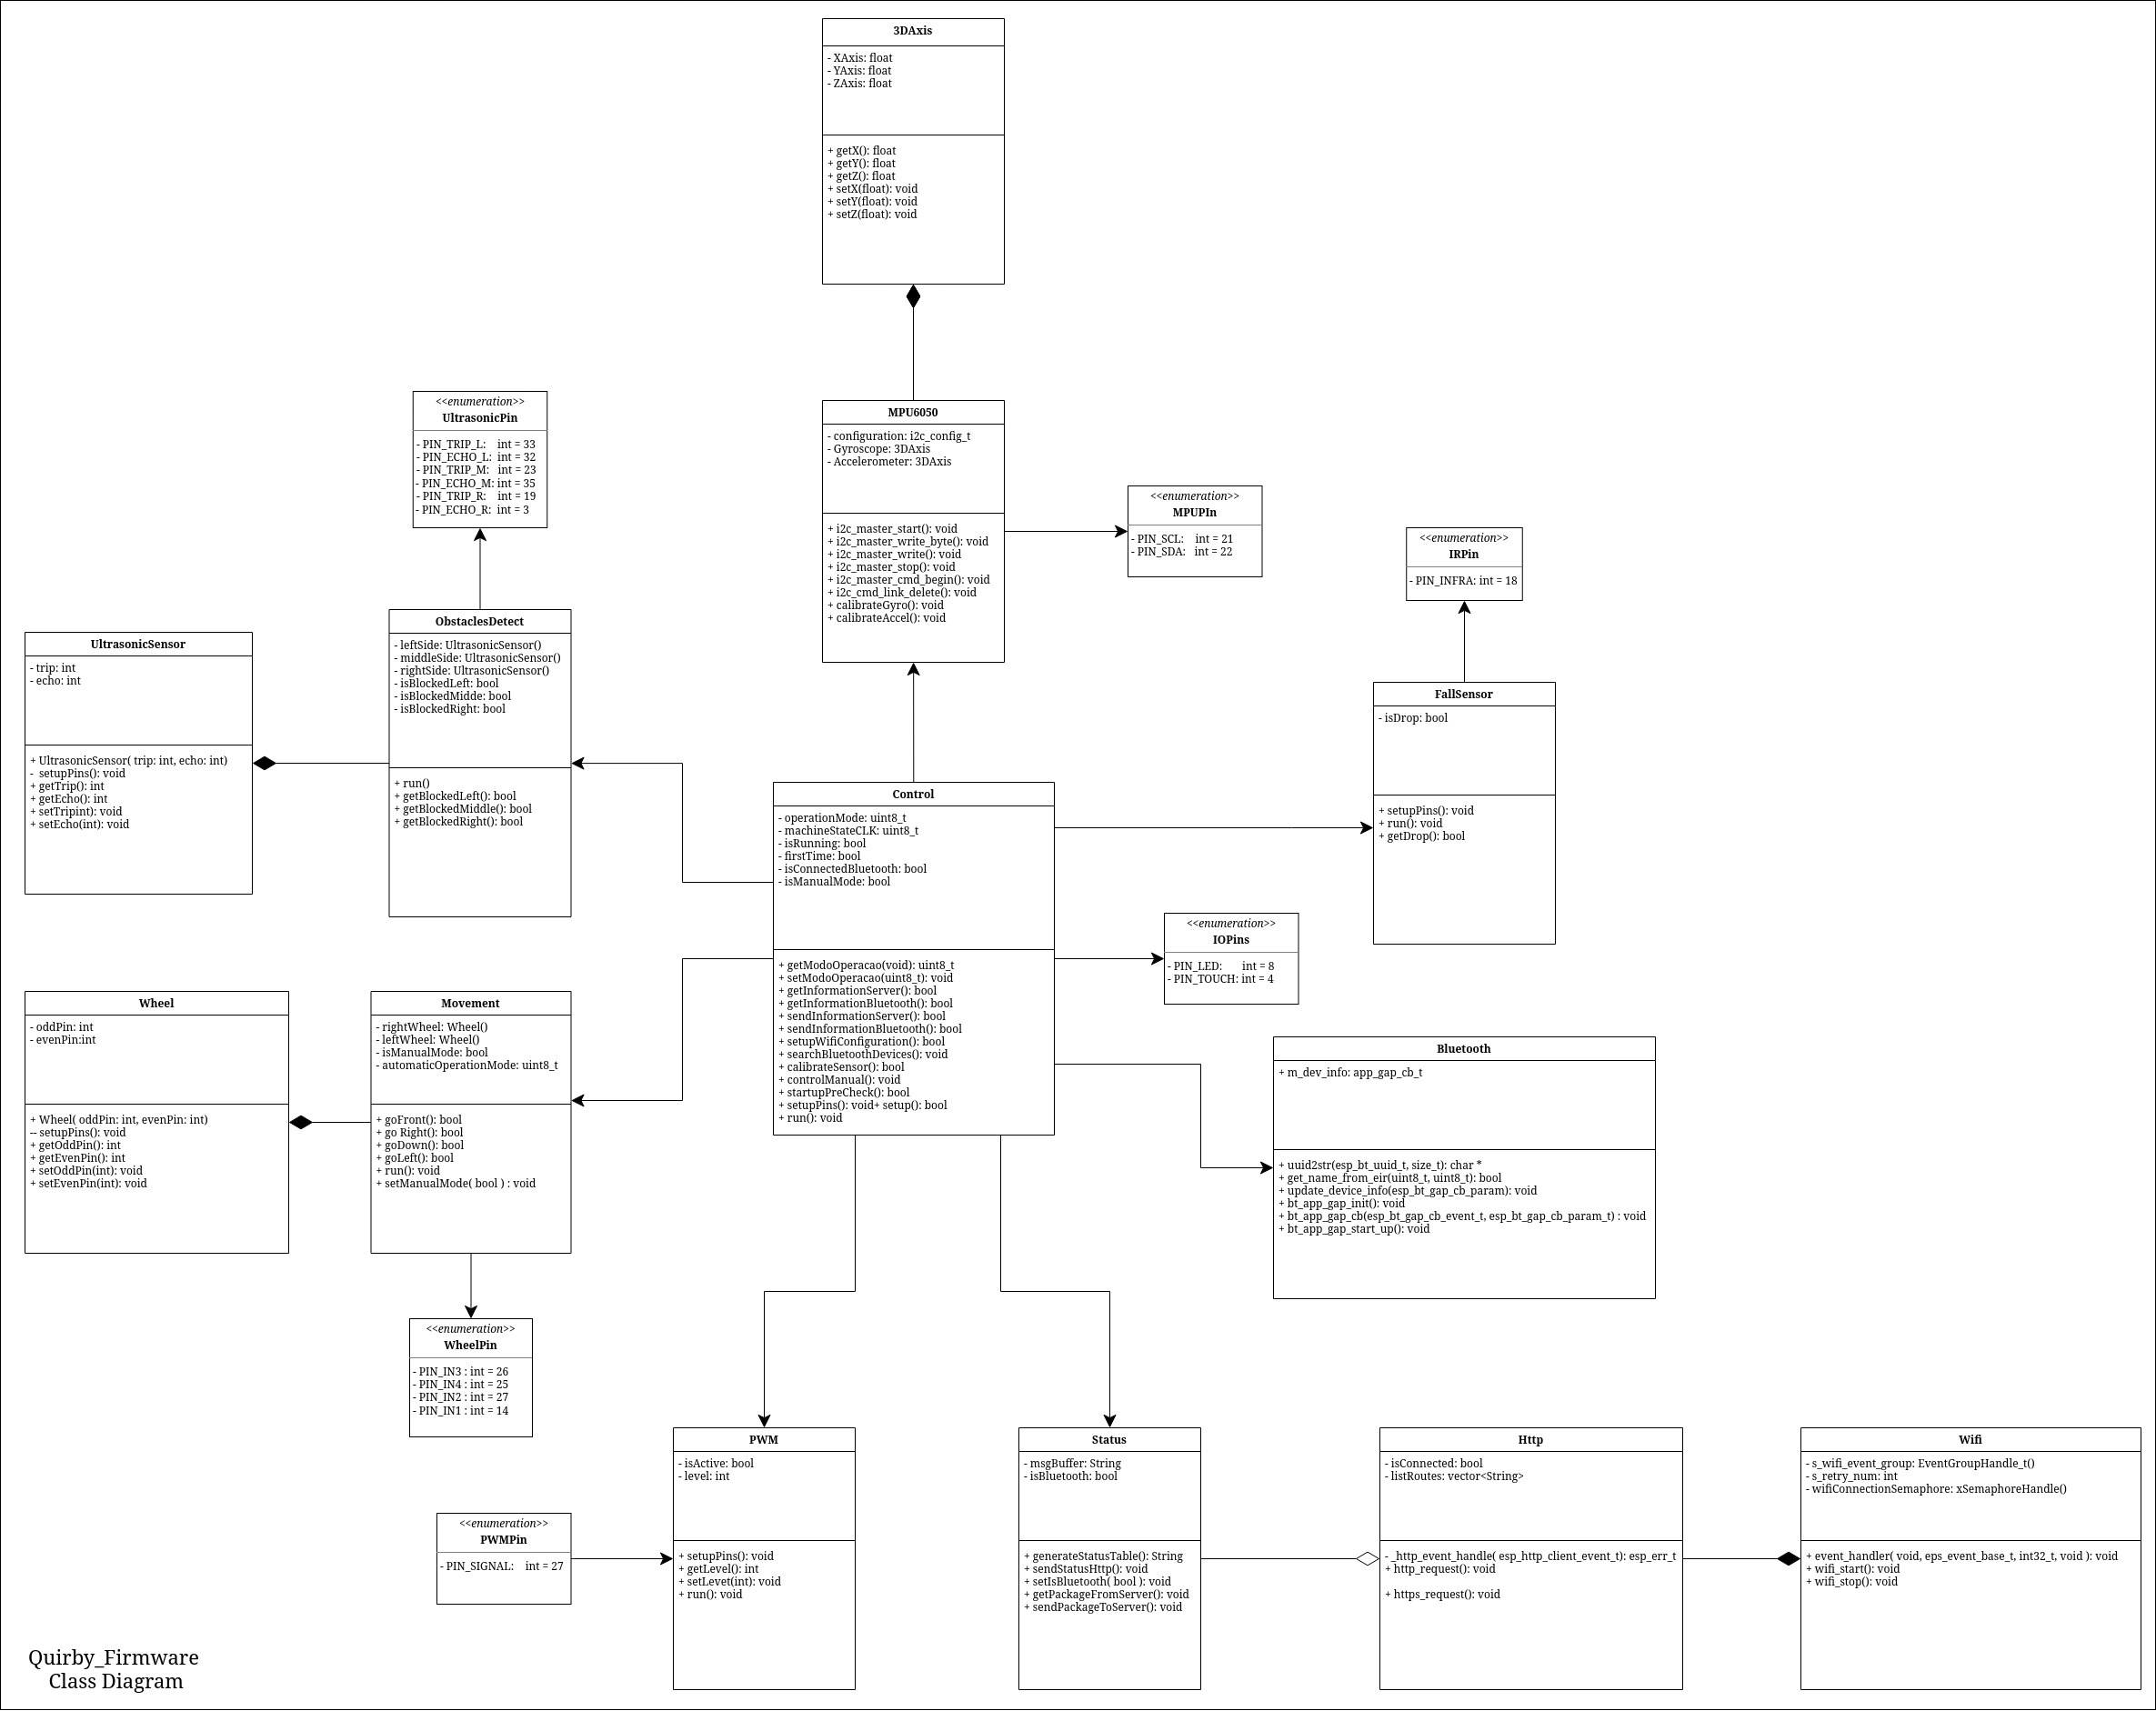
\includegraphics[scale=0.2]{figuras/Quirby_Firmware_Diagrama_de_Classes.jpg}
\caption{Diagrama de Classes do Firmware \\ Fonte: Autoria própria, 2023. }
\textit{Para melhor visualização, acesse a imagem externamente clicando \href{https://drive.google.com/file/d/1FaDMcYj23tRlHez7_HY8dnomueZytGaC/view?usp=sharing}{aqui}.}
\label{diagramaClasseFirm}
\end{figure}

O Apêndice \ref{diagramaFirmware}, contém em detalhes todo o fluxograma em relação aos diagrama de sequência e também a estrutura de comunicação entre os pacotes. 